\begin{scanpage}{0170}{152}
\begin{center}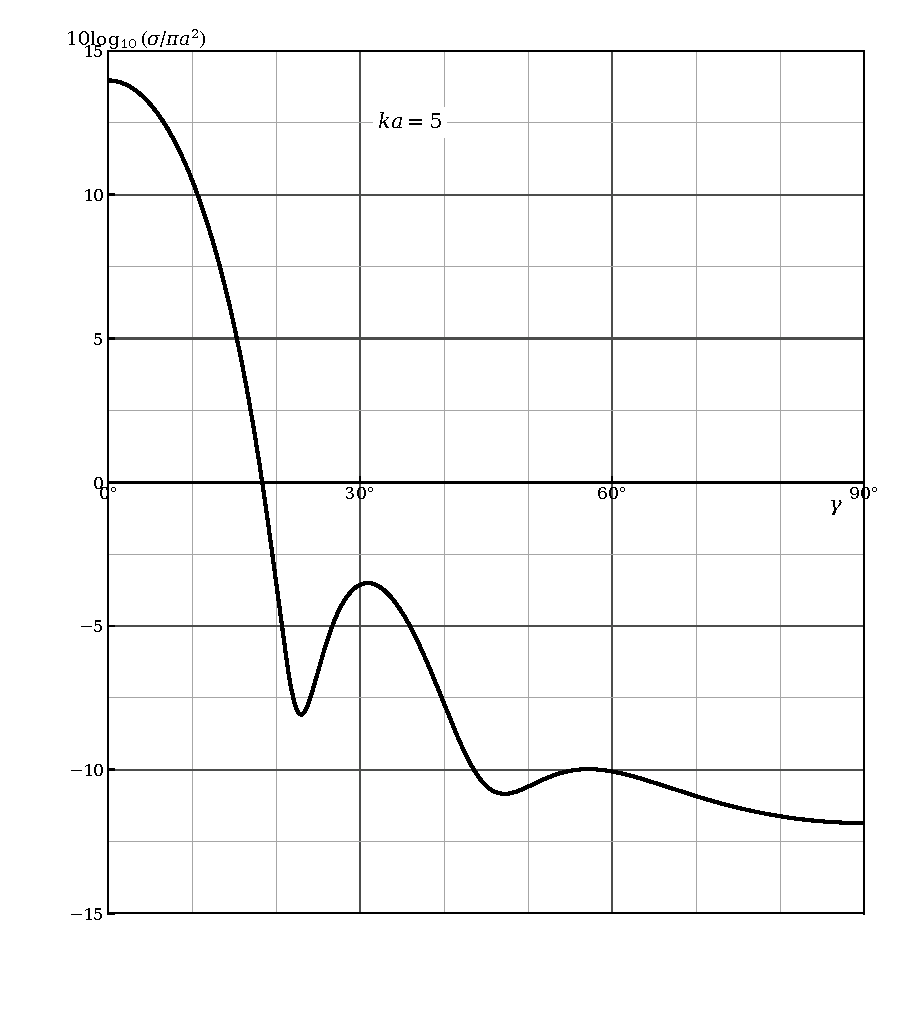
\includegraphics[width=.62\linewidth]{images/recreated/c-0170-fig66.pdf}\par
Figure 66. The calculated diagram of a disk's effective scattering surface when the plane wave's electric vector is perpendicular to the incident plane.
\end{center}
the uniform part of the current (the physical optics approach). Curve 3 corresponds to the field from the uniform and nonuniform parts of the current, but without the interaction of the edges. Curve 4 corresponds to the field with consideration of secondary diffraction. As is seen from these graphs, consideration of the edge interaction refines the previous approximation and ensures better agreement with the rigorous theory results.

The problem of secondary diffraction by a cylinder may be solved by a similar method. However, considering that the corrections which
\end{scanpage}
